\chapter{Riconoscimento gesture}

\section{Introduzione alle tecniche utilizzate}

Ci siamo occupati di riconoscere due tipologie di gesture: statiche e dinamiche.\\
Gli strumenti utilizzati sono stati quelli appena spiegati nel capitolo precedente, come i vettori, 
la velocità e le distanze dei vari punti rispetto al centro del polso, che identifica la nostra origine.\\
La scelta di adottare le distanze dal polso rimane valida perché le dita si possono muovere solo di 180°, gli unici punti su cui porre attenzione sono quelli del pollice che spesso assumono la stessa distanza dal polso con gesture diverse:

\vspace{+ 15 px}
\begin{multicols}{2}
    \begin{multicolfigure}
        \centering
        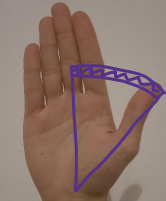
\includegraphics[width=0.956\textwidth]{images/pollici_1.png}
    \end{multicolfigure}
    \columnbreak
    \begin{multicolfigure}
        \centering
        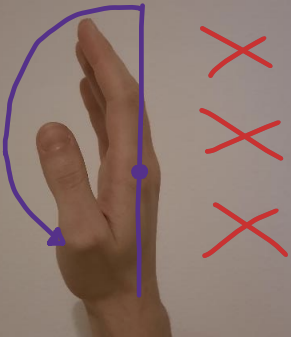
\includegraphics[width=\textwidth]{images/pollici_2.png}
    \end{multicolfigure} 
\end{multicols}
\vspace{+ 15 px}

\noindent Quindi la distanza punto-centro polso può essere utilizzata come discriminante, questione diversa sarebbe stata se le dita fossero state in grado di muoversi liberamente a 360°. Infine, ritornando alla problematica del pollice, in alcuni casi è stato necessario verificare se un dito preso in analisi fosse dritto o piegato.\\
\newpage
\noindent Infine, in alcuni casi, è stato necessario verificare se un dito preso in analisi fosse dritto o piegato; per farlo tracciamo una linea immaginaria tra i due estremi di interesse e verifichiamo quanto ciascun punto in mezzo si discosta dalla linea immaginaria.

\noindent Piccola anticipazione necessaria ma che verrà trattata meglio nel prossimo capitolo: per le distanze sono state adottate le proporzioni prendendo come punto di riferimento la lunghezza definita dal polso, lungo tutta la falange, fino ad arrivare alla punta del dito medio. In questa maniera non si lavora su lunghezze assolute e si permette all’applicazione di riconoscere gesti di persone diverse. Inoltre questa lunghezza è stata suddivisa in 70 livelli, numero non a caso ma scelto empiricamente in base alla precisione/affidabilità dei dati offerti da MediaPipe: un numero di livelli maggiore significava quantizzare le distanze rilevate dalla libreria conservando molta della loro precisione; non possiamo  affidarci troppo ai dati offerti, ma considerare un certo margine di errore, andando ad introdurlo nella fase di quantizzazione(COLLEGAMENTO AL CAPITOLO DEI LIVELLI DI RIK). In seguito vediamo le tecniche adottate per ciascuna gesture, raggruppate per tipologia:

\newpage
\section{Algoritmi per il riconoscimento}
Nella sezione che segue verrà mostrata la logica applicativa dietro il riconoscimento di ogni gesture.

\subsection{Gesture statiche}
Per tutte le gesture appartenenti a questa categoria è stata utilizzata la metodologia \textbf{a livelli}.
\subsubsection{Thumb up}
Per riconoscere il "\textit{pollice in su}" abbiamo scelto di prendere in analisi le punte di ogni dito della mano. Sono stati quindi misurati e testati empiricamente dei livelli che rappresentassero il movimento che volevamo. 
In particolare, abbiamo constatato che questi valori fossero i seguenti:
\begin{multicols}{2}
    \begin{multicolfigure}
        \centering
        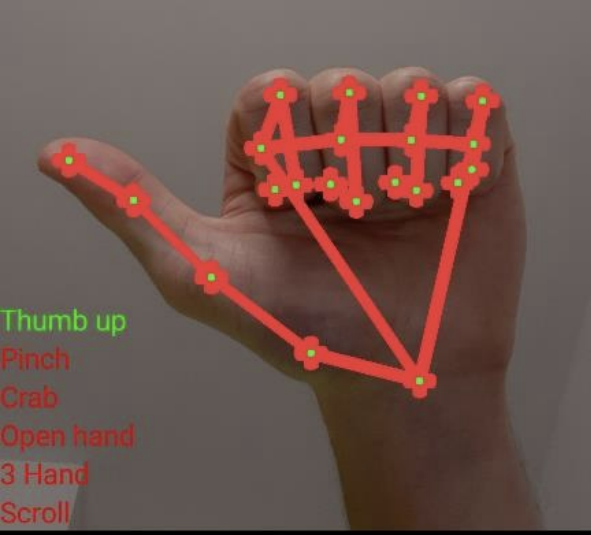
\includegraphics[width=\textwidth]{images/thumb_up.png}
    \end{multicolfigure}
    \columnbreak
    \begin{itemize}
        \item \texttt{HandPoints.THUMB\_TIP}: 52
        \item \texttt{HandPoints.INDEX\_TIP}: 35
        \item \texttt{HandPoints.MIDDLE\_TIP}: 29
        \item \texttt{HandPoints.RING\_TIP}: 27
        \item \texttt{HandPoints.PINKY\_TIP}: 29
    \end{itemize} 
\end{multicols}

\noindent Abbiamo poi introdotto un errore di 8 livelli per avere un buon trade-off tra precisione della posizione e flessibilità del riconoscimento.\\
\\
\noindent Infine, è stato inserito un ulteriore controllo per verificare che il pollice sia in posizione diritta (esteso). Questo è necessario per il motivo detto prima, secondo il quale i \textit{landmarks} del pollice spesso assumono la stessa distanza dal polso pur essendo in posizioni diverse.

\newpage
\subsubsection{Three Hand}
Per il simbolo "\textit{tre}", la tecnica è stata analoga al caso precedente.\\
I valori rilevati come punto di riferimento sono stati i seguenti:
\begin{multicols}{2}
    \begin{multicolfigure}
        \centering
        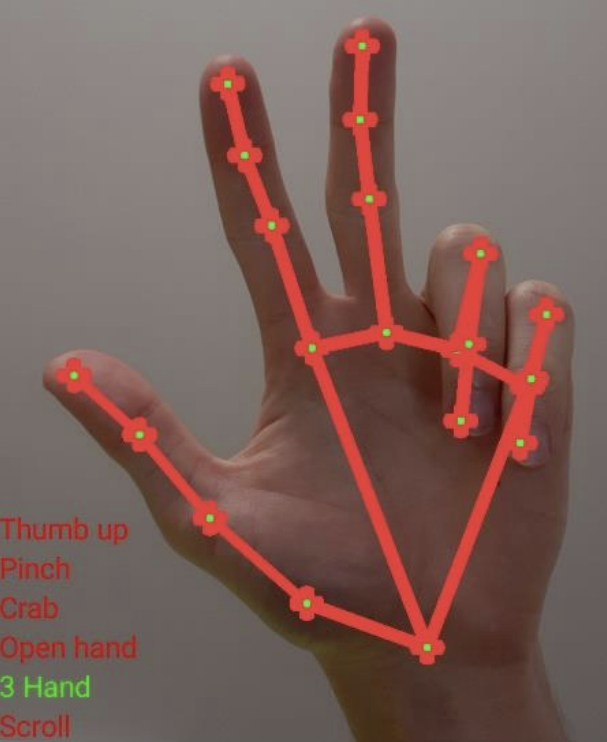
\includegraphics[width=\textwidth]{images/three_hand.png}
    \end{multicolfigure}
    \columnbreak
    \begin{itemize}
        \item \texttt{HandPoints.THUMB\_TIP}: 48
        \item \texttt{HandPoints.INDEX\_TIP}: 65
        \item \texttt{HandPoints.MIDDLE\_TIP}: 67
        \item \texttt{HandPoints.RING\_TIP}: 39
        \item \texttt{HandPoints.PINKY\_TIP}: 32
    \end{itemize} 
\end{multicols}
\noindent Anche qui, viene effettuato il controllo sul fatto che il pollice sia esteso.


\subsubsection{Four Hand}
Anche per il simbolo "\textit{quattro}", la tecnica è stata la stessa.\\
I valori rilevati come punto di riferimento sono stati i seguenti:
\begin{multicols}{2}
    \begin{multicolfigure}
        \centering
        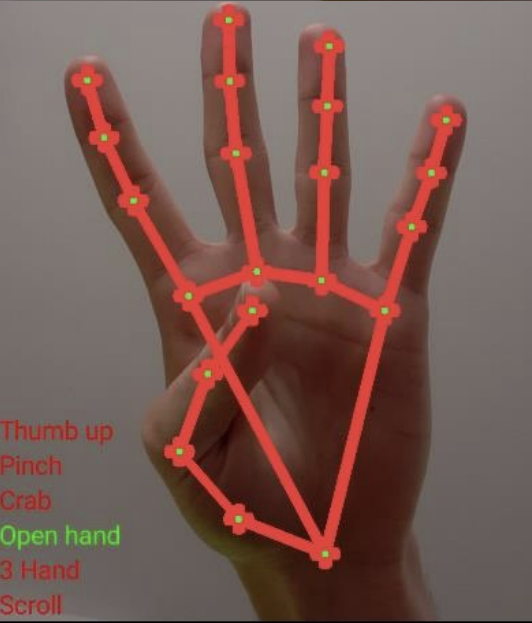
\includegraphics[width=\textwidth]{images/four_hand.png}
    \end{multicolfigure}
    \columnbreak
    \begin{itemize}
        \item \texttt{HandPoints.THUMB\_TIP}: 42
        \item \texttt{HandPoints.INDEX\_TIP}: 63
        \item \texttt{HandPoints.MIDDLE\_TIP}: 67
        \item \texttt{HandPoints.RING\_TIP}: 62
        \item \texttt{HandPoints.PINKY\_TIP}: 54
    \end{itemize} 
\end{multicols}


\subsection{Gesture dinamiche}

\subsubsection{Crab}
A differenza dei casi appena visti, qui ci si occupa di verificare che le punte del pollice e dell'indice si tocchino e che il pollice sia piegato.\\
Oltre a rilevare la gesture era necessario sapere di quanto si spostava la punta del pollice mentre il riconoscimento del gesto era valido. 
Essendo che Mediapipe offre anche dei valori già in forma di coordinate normalizzate rispetto allo schermo (\texttt{multiHandLandmarks}), è stato sufficiente andarsi a costruire un vettore con partenza il primo punto rilevato appena la gesture viene riconosciuta e come destinazione l'ultimo punto rilevato.\\
In questo modo abbiamo tracciato un vettore direzionato a rappresentare il nostro movimento.
\begin{figure}[H]
    \centering
    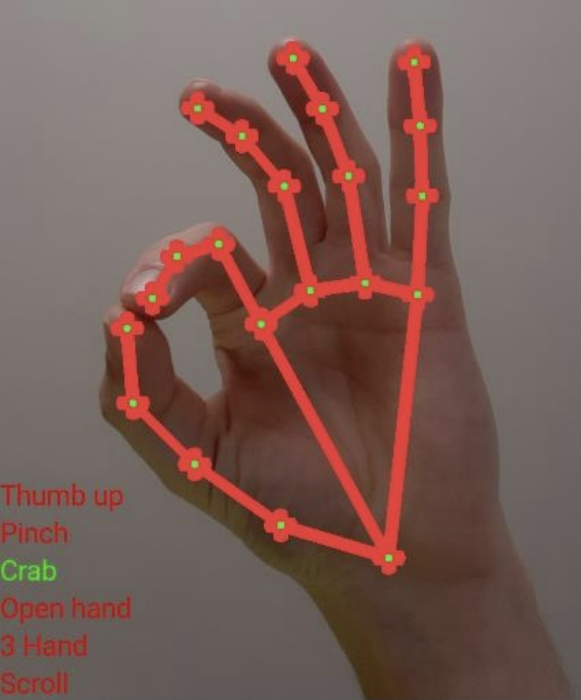
\includegraphics[width=0.6\textwidth]{images/crab.png}
\end{figure}
\noindent Il protocollo di riconoscimento impone che si inizi con la mano aperta, si chiudano pollice ed indice e li si muovano poi per definire il vettore di spostamento.

\newpage
\subsubsection{Pinch}
Per questa gesture viene utilizzata una metodologia ibrida.\\
Si verifica che la posizione delle punte delle dita medio, anulare e mignolo siano coerenti (a fronte di un margine di errore) coi seguenti livelli:
\begin{itemize}
    \item \texttt{HandPoints.MIDDLE\_TIP}: 29
    \item \texttt{HandPoints.RING\_TIP}: 27
    \item \texttt{HandPoints.PINKY\_TIP}: 29
\end{itemize} 
\noindent Succesivamente, si rileva la distanza tra la punta dell'indice e del pollice.
\begin{multicols}{2}
    \begin{multicolfigure}
        \centering
        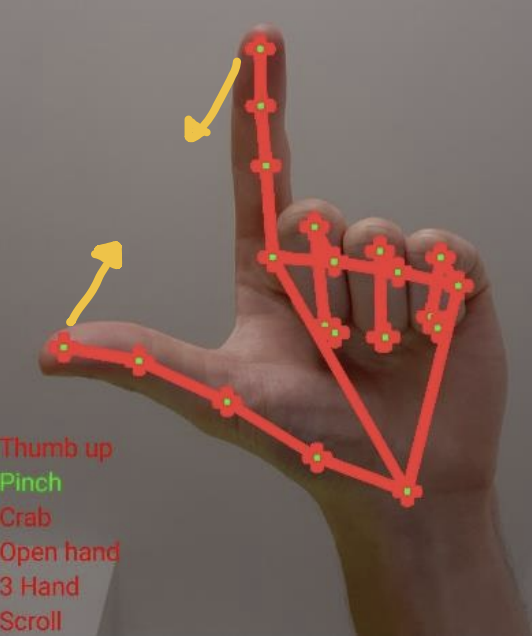
\includegraphics[width=0.9\textwidth]{images/pinch_1.png}
    \end{multicolfigure}
    \columnbreak
    \begin{multicolfigure}
        \centering
        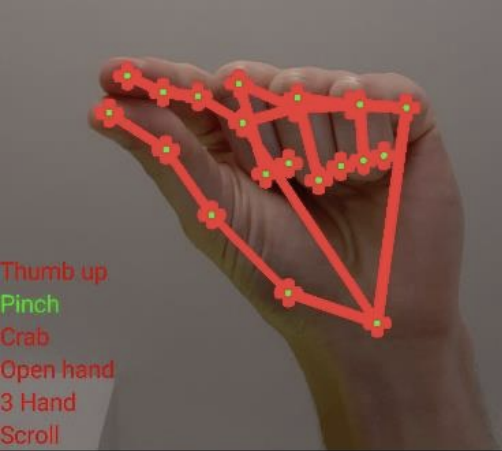
\includegraphics[width=1.1\textwidth]{images/pinch_2.png}
    \end{multicolfigure} 
\end{multicols}
\noindent Il protocollo di riconoscimento impone che si inizi con la mano a forma di \texttt{L} (come nell'immagine a sinistra).

\newpage
\subsubsection{Scroll}
Viene utilizzato il concetto di velocità.\\
Come verifica preliminare, si controlla che indice e medio siano le uniche due dita alzate (ovvero che i loro \textit{landmarks} siano quelli con una coordinata \texttt{y} minore). Inoltre, si verifica che il pollice sia piegato per non entrare in conflitto con la gesture \texttt{pinch}.\\
\\
\noindent Al primo riconoscimento, passati i controlli precedenti, si verifica che la posizione della punta del dito indice si trovi su un lato dello schermo e, in caso affermativo, si memorizza il valore della \texttt{x} della punta dell'indice per poi poterlo confrontare in un secondo rilevamento.\\
Infatti, se la punta dell'indice risulta essersi mossa nel lato opposto dello schermo con una velocità superiore ad una certa soglia, la gesture è riconosciuta.
\begin{multicols}{2}
    \begin{multicolfigure}
        \centering
        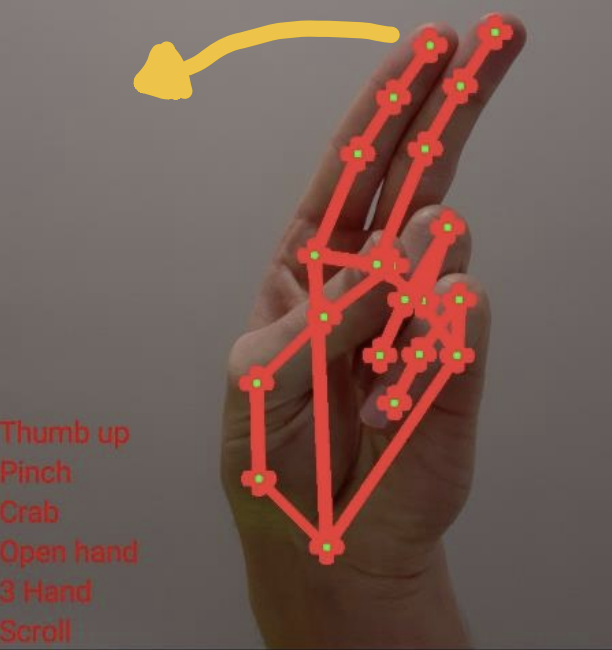
\includegraphics[width=\textwidth]{images/scroll_1.png}
    \end{multicolfigure}
    \columnbreak
    \begin{multicolfigure}
        \centering
        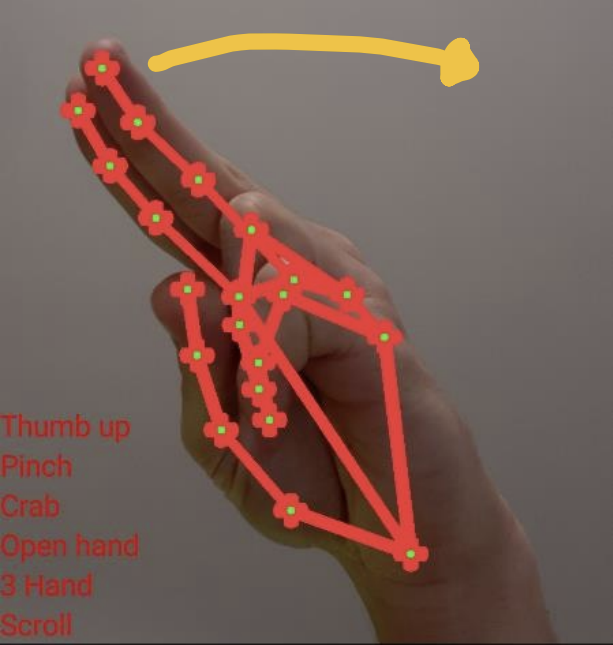
\includegraphics[width=\textwidth]{images/scroll_2.png}
    \end{multicolfigure} 
\end{multicols}